\begin{figure}[hpt!]
\centering
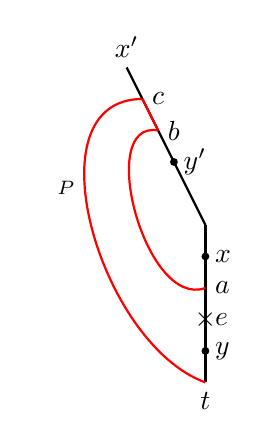
\begin{tikzpicture}[scale=2]
\begin{scope}
\coordinate (s) at (-0.5,2);
\coordinate (s1) at (0.5,2);
\coordinate (w) at (0,1);
\coordinate (t) at (0,0);
\coordinate (x) at (0,0.8);
\coordinate (y) at (0,0.2);
\coordinate (y1) at (-0.2,1.4);
\coordinate (i1) at (-0.4,1.8);
\coordinate (i2) at (-0.3,1.6);
\coordinate (a) at (0,0.6);
\coordinate (v) at (0,0.4);



\draw[thick](s)--(w);
%\draw[thick](s1)--(w);
\draw[thick](w)--(t);
\node[above] at (s){$x'$};
%\node[above] at (s1){$s$};
\node[below] at (t){$t$};

\node[right] at (a){$a$};

%\node[right] at (w){$w$};
\node[right] at (i1){$c$};
\node[right] at (i2){$b$};


\draw[red,thick] (a) to[out=200,in=170]
(i2);
\draw[red,thick](i1)--(i2);
\draw[red,thick] (i1) to[out=180,in=160]node[pos=0.4,left,black]{\scriptsize{$P$}}  (t);
\node at (v){$\times$};
\node[right] at (v){$e$};
\draw (y) node[fill,circle,scale=0.3]{};
\node[right] at (y){$y$};
\draw (x) node[fill,circle,scale=0.3]{};
\node[right] at (x){$x$};
\draw (y1) node[fill,circle,scale=0.3]{};
\node[right] at (y1){$y'$};
\end{scope}
\end{tikzpicture}
\caption{The path $P$ merges with another segment $x'y'$  and then diverges.}
\label{fig:feature}

\end{figure}
